\documentclass[tikz,border=2pt]{standalone}
\usepackage[T1]{fontenc}
\usepackage{helvet}
\usepackage{amsmath}
\renewcommand{\familydefault}{\sfdefault}
\usetikzlibrary{arrows.meta,calc}
\definecolor{ink}{HTML}{1F1F1F}
\definecolor{accent}{HTML}{1B6B5F}
\definecolor{accentfill}{HTML}{DCEBE4}
\tikzset{every node/.style={font=\sffamily\fontsize{9}{11}\selectfont,text=ink},base/.style={draw=ink,line width=.65pt,align=center,inner sep=2pt},tensor/.style={base,rounded corners=1.6pt,fill=white},transform/.style={base,fill=black!4},state/.style={tensor,double,double distance=.6pt},junction/.style={base,circle,fill=white,inner sep=0pt},highlight/.style={draw=accent,fill=accentfill},edge/.style={draw=ink,line width=.65pt,-{Stealth[length=1.6mm]}},feedback/.style={dashed},control/.style={densely dotted},edgefocus/.style={draw=accent},note/.style={font=\sffamily\fontsize{8}{9}\selectfont,align=center}}
\begin{document}
\begin{tikzpicture}[x=1mm,y=-1mm]

\path[use as bounding box] (0,0) rectangle (258,59);
\node[tensor,text width=44mm,minimum height=43mm] (forking) at (25,26) {};
\node[tensor,text width=44mm,minimum height=43mm] (ngram) at (94,26) {};
\node[tensor,text width=44mm,minimum height=43mm] (novel) at (163,26) {};
\node[tensor,highlight,text width=44mm,minimum height=43mm] (sharpening) at (232,26) {};
\draw[edge,edgefocus] (forking.east) -- (ngram.west);
\node[note,fill=white,inner sep=1pt] at (59.5,20) {{\bfseries OPHIS}\\+ removal};
\draw[edge,edgefocus] (ngram.east) -- (novel.west);
\node[note,fill=white,inner sep=1pt] at (128.5,20) {{\bfseries Frequency}\\experiments};
\draw[edge,edgefocus] (novel.east) -- (sharpening.west);
\node[note,fill=white,inner sep=1pt] at (197.5,20) {{\bfseries Replay}\\dynamics};
\node[note] at (25,12) {{\bfseries\fontsize{10.5}{12}\selectfont Forking}};
\node[note] at (25,27) {\begin{tikzpicture}[x=1mm,y=1mm,baseline=0mm]\draw[black!35,line width=.4pt] (0,0)--(0,13) (0,0)--(32,0);\draw[black!45,line width=1pt] (1,11)..controls (7,5) and (12,4)..(15,4)..controls (22,2) and (26,1)..(30,1);\draw[accent,line width=1.1pt] (1,11)..controls (7,5) and (12,4)..(15,4)--(16,7)--(23,7.5)--(24,10)--(30,10.5);\draw[black!25,dashed] (15,0)--(15,12);\node[font=\tiny,text=accent] at (28,13) {val};\node[font=\tiny,text=black!55] at (28,-2) {train};\end{tikzpicture}};
\node[note] at (25,43) {{\small Losses split under replay}};
\node[note] at (94,12) {{\bfseries\fontsize{10.5}{12}\selectfont $n$-gram memory}};
\node[note] at (94,27) {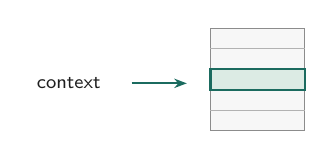
\begin{tikzpicture}[x=1mm,y=1mm,baseline=0mm]\node[font=\scriptsize] at (5,6) {context};\draw[edge,draw=accent] (13,6)--(20,6);\draw[draw=black!45,fill=black!3] (23,0) rectangle (35,13);\fill[accentfill] (23,5) rectangle (35,8);\foreach \y in {2.6,5.2,7.8,10.4}{\draw[black!30,line width=.35pt] (23,\y)--(35,\y);}\draw[accent,line width=.8pt] (23,5.2) rectangle (35,7.8);\end{tikzpicture}};
\node[note] at (94,43) {{\small Removing tables removes\\the rapid divergence}};
\node[note] at (163,12) {{\bfseries\fontsize{10.5}{12}\selectfont Novel continuations}};
\node[note] at (163,27) {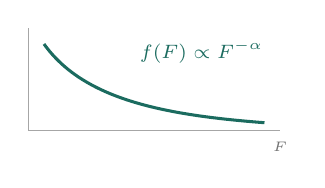
\begin{tikzpicture}[x=1mm,y=1mm,baseline=0mm]\draw[black!35,line width=.4pt] (0,0)--(0,13) (0,0)--(32,0);\draw[accent,line width=1.1pt] (2,11)..controls (7,4) and (17,2)..(30,1);\node[font=\scriptsize,text=accent] at (22,10) {$f(F)\propto F^{-\alpha}$};\node[font=\tiny,text=black!55] at (32,-2) {$F$};\end{tikzpicture}};
\node[note] at (163,43) {{\small Rare contexts leave\\more continuations unseen}};
\node[note] at (232,12) {{\bfseries\fontsize{10.5}{12}\selectfont Local sharpening}};
\node[note] at (232,27) {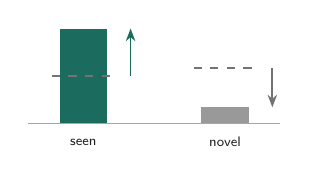
\begin{tikzpicture}[x=1mm,y=1mm,baseline=0mm]\draw[black!35,line width=.4pt] (0,0)--(32,0);\fill[accent] (4,0) rectangle (10,12);\draw[black!55,dashed,line width=.6pt] (3,6)--(11,6);\draw[edge,draw=accent] (13,6)--(13,12);\fill[black!40] (22,0) rectangle (28,2);\draw[black!55,dashed,line width=.6pt] (21,7)--(29,7);\draw[edge,draw=black!55] (31,7)--(31,2);\node[font=\tiny] at (7,-2.4) {seen};\node[font=\tiny] at (25,-2.4) {novel};\end{tikzpicture}};
\node[note] at (232,43) {{\small Replay favors seen targets\\and crowds out alternatives}};
\node[note] at (59.5,54) {\textcolor{black!55}{Which component?}};
\node[note] at (128.5,54) {\textcolor{black!55}{Which predictions?}};
\node[note] at (197.5,54) {\textcolor{black!55}{Why does replay hurt?}};
\node[note] at (232,4) {\textcolor{accent}{\scriptsize PROPOSED MECHANISM}};
\end{tikzpicture}
\end{document}
